% Advisor report (up to seven pages): AMOC adjoint sensitivity in the 2° OMIP ocean, state as of mid-November 2026.
% Build with `latexmk -pdf omip_amoc_adjoint_advisor_report.tex` in this directory. Detail: omip_amoc_adjoint.tex,
% ../REACTANT_ENZYME_ISSUES.md and the repository-root STATUS.md.
\documentclass[10pt]{article}

\usepackage[margin=0.8in]{geometry}
\usepackage{amsmath, amssymb}
\usepackage{booktabs}
\usepackage{graphicx}
\usepackage{hyperref}
\usepackage{siunitx}
\usepackage{enumitem}
\usepackage{caption}
\usepackage{float}
\usepackage{titlesec}
\titlespacing*{\section}{0pt}{9pt}{3pt}
\titlespacing*{\subsection}{0pt}{6pt}{2pt}
\setlist{nosep, leftmargin=1.3em}
\captionsetup{font=small, skip=4pt}
\setlength{\parskip}{4pt}
\setlength{\parindent}{0pt}

\newcommand{\gvec}{\mathbf{g}}

\title{\vspace{-2em}\textbf{Adjoint sensitivity of the AMOC at \ang{26.5}N in a differentiable OMIP ocean}\\[2pt]
       \large Progress report\vspace{-0.4em}}
\date{\today\vspace{-1em}}

\begin{document}
\maketitle

\section{Summary}

The goal is the sensitivity of the Atlantic overturning at \ang{26.5}N to the surface forcing that precedes it,
as in Pillar et al.\ (2016), computed with the Enzyme reverse-mode adjoint of a Reactant-compiled
\textsc{Oceananigans} ocean (NumericalEarth's OMIP configuration, 2\textdegree, 20 levels).
\begin{enumerate}
  \item \textbf{The cost does not grow with window length.} One time step and its reverse pass are compiled once,
        in about \SI{28}{min}, and run on a binomial (Revolve) checkpoint schedule. A compiled gradient then costs
        \SI{104}{s} for 30 days with 3-hourly JRA55 forcing, and \SI{15}{min} for a year with monthly ECCO4 fluxes.
  \item \textbf{The adjoint is exact.} Finite differences agree with it to \numrange{e-9}{e-8} at 8, 84 and 360
        steps where the objective is smooth. It also verifies after the move to Oceananigans 0.117.2.
  \item \textbf{The objective is only piecewise smooth past about a day.} Discrete switches in the forward model
        make it jump by \SIrange{e-7}{e-3}{Sv}. At finite amplitude the gradient still predicts the 30-day response
        to within \SIrange{0.05}{2}{\percent}.
  \item \textbf{CATKE must be frozen in the adjoint beyond a month.} At 90 days the full adjoint is NaN in every
        wet cell; with frozen mixing it is finite and within \SI{2.2}{\percent} of finite differences.
  \item \textbf{First Pillar-style lead-time maps} (90 days, ECCO4 fluxes): an Ekman band, then boundary and
        equatorial waveguides spreading with lead, as in Pillar's $-1$ and $-3$ month rows.
  \item \textbf{Windows of 180 days and longer blow up, even with frozen mixing.} The cause is in the forward
        trajectory: grid-scale noise grows in fronts and convective regions, and SST drifts \SI{3}{\celsius}
        from ECCO4 under fixed fluxes. Turning off GM/Redi or WENO does not fix it. The time step does not seem to be
        the cause. \emph{Decision needed:} SST/SSS feedback on the fluxes, explicit horizontal diffusion, or both
        (Section~\ref{sec:next}).
\end{enumerate}

\section{Model and problem}

\begin{center}\small
\begin{tabular}{@{}lp{0.78\textwidth}@{}}
\toprule
Grid & \textsc{TripolarGrid} $180\times60\times20$ ($\approx\ang{2}$), exponential spacing to \SI{5500}{m}, ETOPO bathymetry,
       immersed boundary; a $360\times180\times20$ (\ang{1}) version is queued \\
Dynamics & hydrostatic Boussinesq, TEOS-10; split Runge--Kutta 3, $\Delta t = \SI{2}{h}$; split-explicit free surface \\
Closures & CATKE vertical mixing; GM/Redi ($\kappa = \SI{800}{m^2/s}$); biharmonic viscosity; WENO advection \\
Forcing A & JRA55 repeat-year 3-hourly atmosphere and OMIP-2 bulk formulae, from the WOA state at rest; control:
            the \SI{10}{m} winds on every slice ($\sim 10^8$ controls for 30 days) \\
Forcing B & ECCO4 monthly wind stress, net heat flux and net freshwater flux, from the 1993-01 ECCO4 state; control: all
            four fluxes on every monthly slice (Pillar's controls) \\
Objective & residual overturning $\psi$ at \SI{1000}{m} across a staircase of faces along \ang{26.5}N, \ang{80}W--\ang{14}W
            (RAPID line); at the window's end (A) or averaged over its last 30 days (B) \\
Software & Float64; Oceananigans 0.117.2 (0.113.5 for the results of Sections~\ref{sec:verification}--\ref{sec:lead}),
           Reactant 0.2.303, Enzyme 0.13.216, Julia 1.12.7; NVIDIA A100 and H100 (TACC Lonestar6) \\
\bottomrule
\end{tabular}
\end{center}

With signed, wet-masked face areas $W$ of the staircase and section area $a_k$,
\begin{equation*}
T_k = \sum_{ij} \big(W^{v}_{ijk} v_{ijk} + W^{u}_{ijk} u_{ijk}\big), \quad
\tilde T_k = T_k - \frac{\sum_{k'} T_{k'}}{\sum_{k'} a_{k'}}\, a_k, \quad
J = -10^{-6} \sum_{k \le k_{\text{ref}}} \tilde T_k \;\;[\si{Sv}].
\end{equation*}
On the tripolar grid a single row drifts from \ang{28}N to \ang{34}N across the Atlantic, so the section follows
the faces nearest \ang{26.5}N. $J$ is linear in the velocities.

\section{Adjoint method}

Five functions are compiled once: the diagnostic refresh, one coupled time step, and the reverse passes of the
refresh, the step and $J$. The host drives them on the Revolve schedule (\texttt{Checkpointing.jl}), with each
checkpoint a host copy of the model's device memory. This replaced two dead ends:
\begin{itemize}
  \item a rolled time loop, where Enzyme's reverse loop carried \SI{73}{GiB} of zero shadow state;
  \item differentiating the whole window as one module, which took \SI{48}{min} to compile at only 2 steps and
        grew with $N$.
\end{itemize}
For the 30-day-mean objective, the adjoint receives an extra seed after each of the last $n_{\text{avg}}$ reverse
steps. Because $J$ is linear, that seed does not depend on the state.

\emph{Frozen mixing} passes CATKE's diffusivities through a stop-gradient, as Pillar et al.\ do with KPP. The forward
model is unchanged, and the adjoint treats mixing as fixed along the trajectory.

\begin{center}\small
\begin{tabular}{@{}lrrrr@{}}
\toprule
& model build & gradient compile & first call & each later gradient \\
\midrule
A, 2 to 360 steps (2 h to 30 days) & 15--24 min & 27--29 min & 37--40 min & \SI{0.8}{s} to \SI{104}{s} \\
B, 90 days / 1 year & 6 min & 28--29 min & 18 / 30 min & \SI{3.4}{min} / \SI{14.5}{min} \\
\bottomrule
\end{tabular}
\end{center}
The fixed first-call cost is host-side, most likely Julia compiling call wrappers for the very large model type.
At \ang{1} one reverse step needs a single \SI{31.8}{GiB} allocation, more than an A100 (\SI{40}{GB}) holds, so the
\ang{1} runs use the \SI{80}{GB} H100 nodes.

\section{Verification}
\label{sec:verification}

\begin{center}\small
\begin{tabular}{@{}p{0.3\textwidth}rp{0.19\textwidth}p{0.36\textwidth}@{}}
\toprule
Window & $J$ [Sv] & Check & Result (relative error) \\
\midrule
A, 1 step & $-14.35$ & Taylor; CPU twin & \num{6e-5}; primal vs.\ twin \num{7.5e-13} \\
A, 2 steps (Revolve) & $-28.56$ & Taylor & \num{2e-7}; cosine to unrolled $\gvec$: $1 - \num{4e-10}$ \\
A, 8 / 84 / 360 steps & & FD scan, 25 octaves & central \numrange{4e-9}{2e-8} where $J$ is smooth \\
B, 8 steps, 4-step average & $-7.59$ & Taylor & \num{7.4e-4} (\num{5.5e-4} unaveraged) \\
B, 90 days, 30-day average & $16.71$ & secants $h = 0.025$--$0.1$ & full adjoint: NaN; frozen: 2.2\,\% \\
\midrule
A, 2 steps, Oceananigans 0.117.2 & $-28.51$ & Taylor & \num{1.6e-4}, error falls $4\times$ per halving of $h$ \\
B, 8 steps, Oceananigans 0.117.2 & $24.13$ & Taylor & \numrange{5e-6}{9e-6} at the smallest $h$; jumps at $h \approx 0.01$ \\
\bottomrule
\end{tabular}
\end{center}

\begin{figure}[H]
\centering
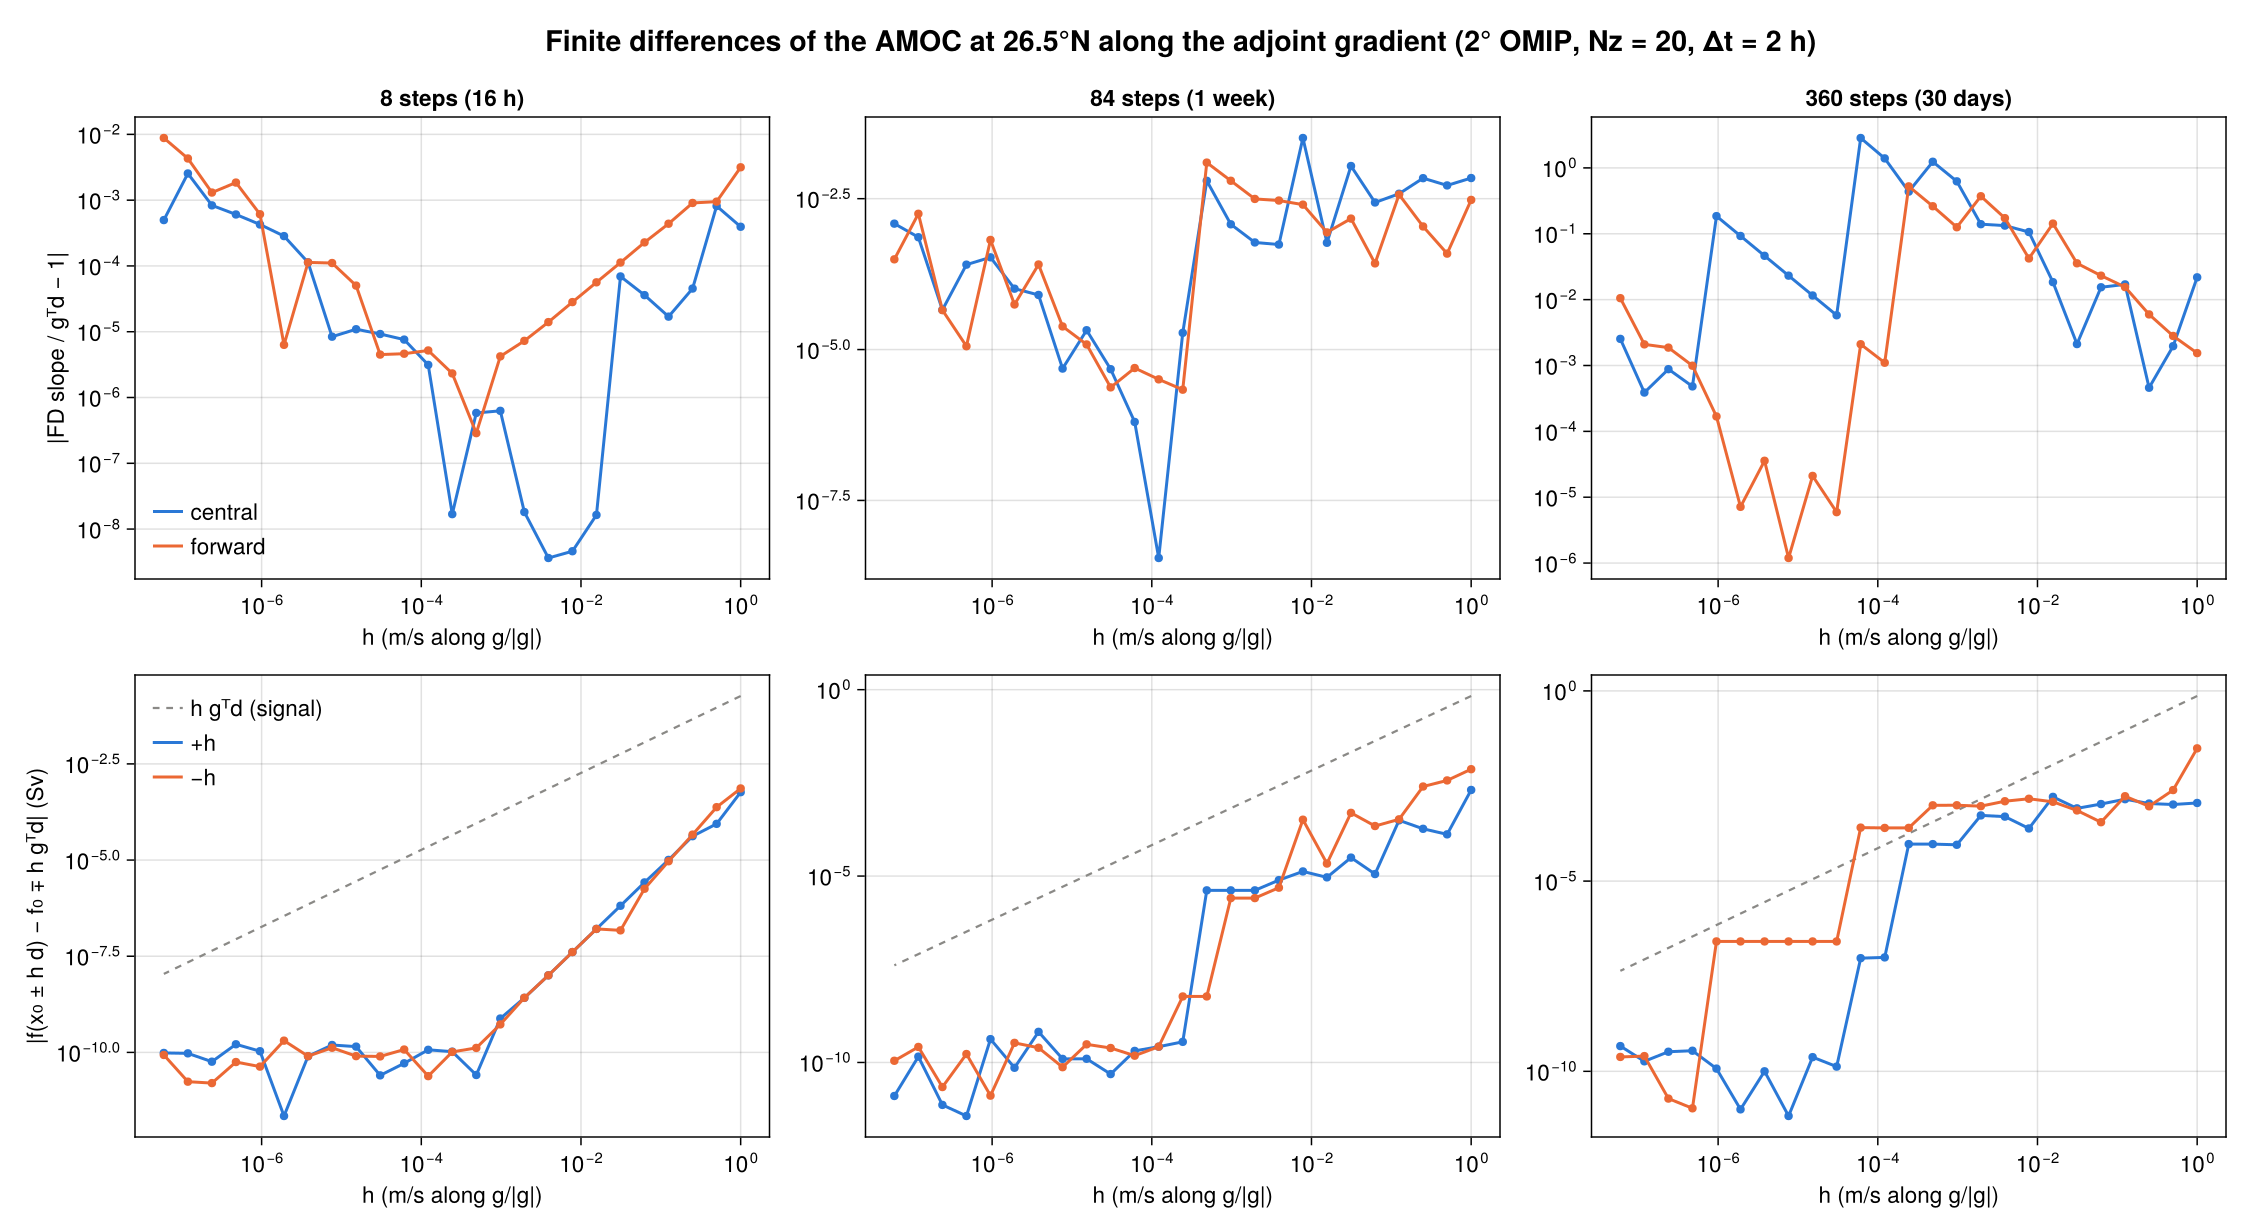
\includegraphics[width=0.78\textwidth]{figures/fd_scans_twodegree_nz20.png}
\caption{Finite differences of $J$ along $d = \gvec/\lVert\gvec\rVert$ at 8, 84 and 360 steps (forcing A). Top:
error of the central and forward differences relative to $\gvec^{\mathsf T}d$. Bottom: residual of the linear
prediction on each side, with the signal $h\,\gvec^{\mathsf T}d$ dashed. A plateau as $h$ shrinks is a jump in $J$.}
\label{fig:fd}
\end{figure}

Below each jump the adjoint and finite differences agree to roundoff, but the smooth neighborhood shrinks with the
window ($h \lesssim \SI{2e-4}{m/s}$ at one week). The adjoint differentiates the branch the forward run took, the
chaotic-adjoint behavior of Lea et al.\ (2000). At finite amplitude ($h = 0.25$--\SI{1}{m/s}) the secant slope
matches $\gvec^{\mathsf T}d$ to \num{4e-4} at 8 steps, \numrange{5e-3}{7e-3} at 84 and \numrange{5e-4}{2e-2} at 360.

\textbf{Frozen against full mixing.} At 84 and 360 steps the frozen gradient has cosine 0.9996 and 0.994 with the
full one. It predicts the finite-amplitude response \SIrange{0.4}{1.7}{\percent} less accurately and saves no time.
Its uniform-wind sums can differ by $2.4\times$, because those sums cancel large values of both signs. At 90 days the
full adjoint is NaN, and only the frozen one is usable.

\section{Results}
\label{sec:lead}

\subsection{Wind sensitivity over 30 days (forcing A)}

\begin{figure}[H]
\centering
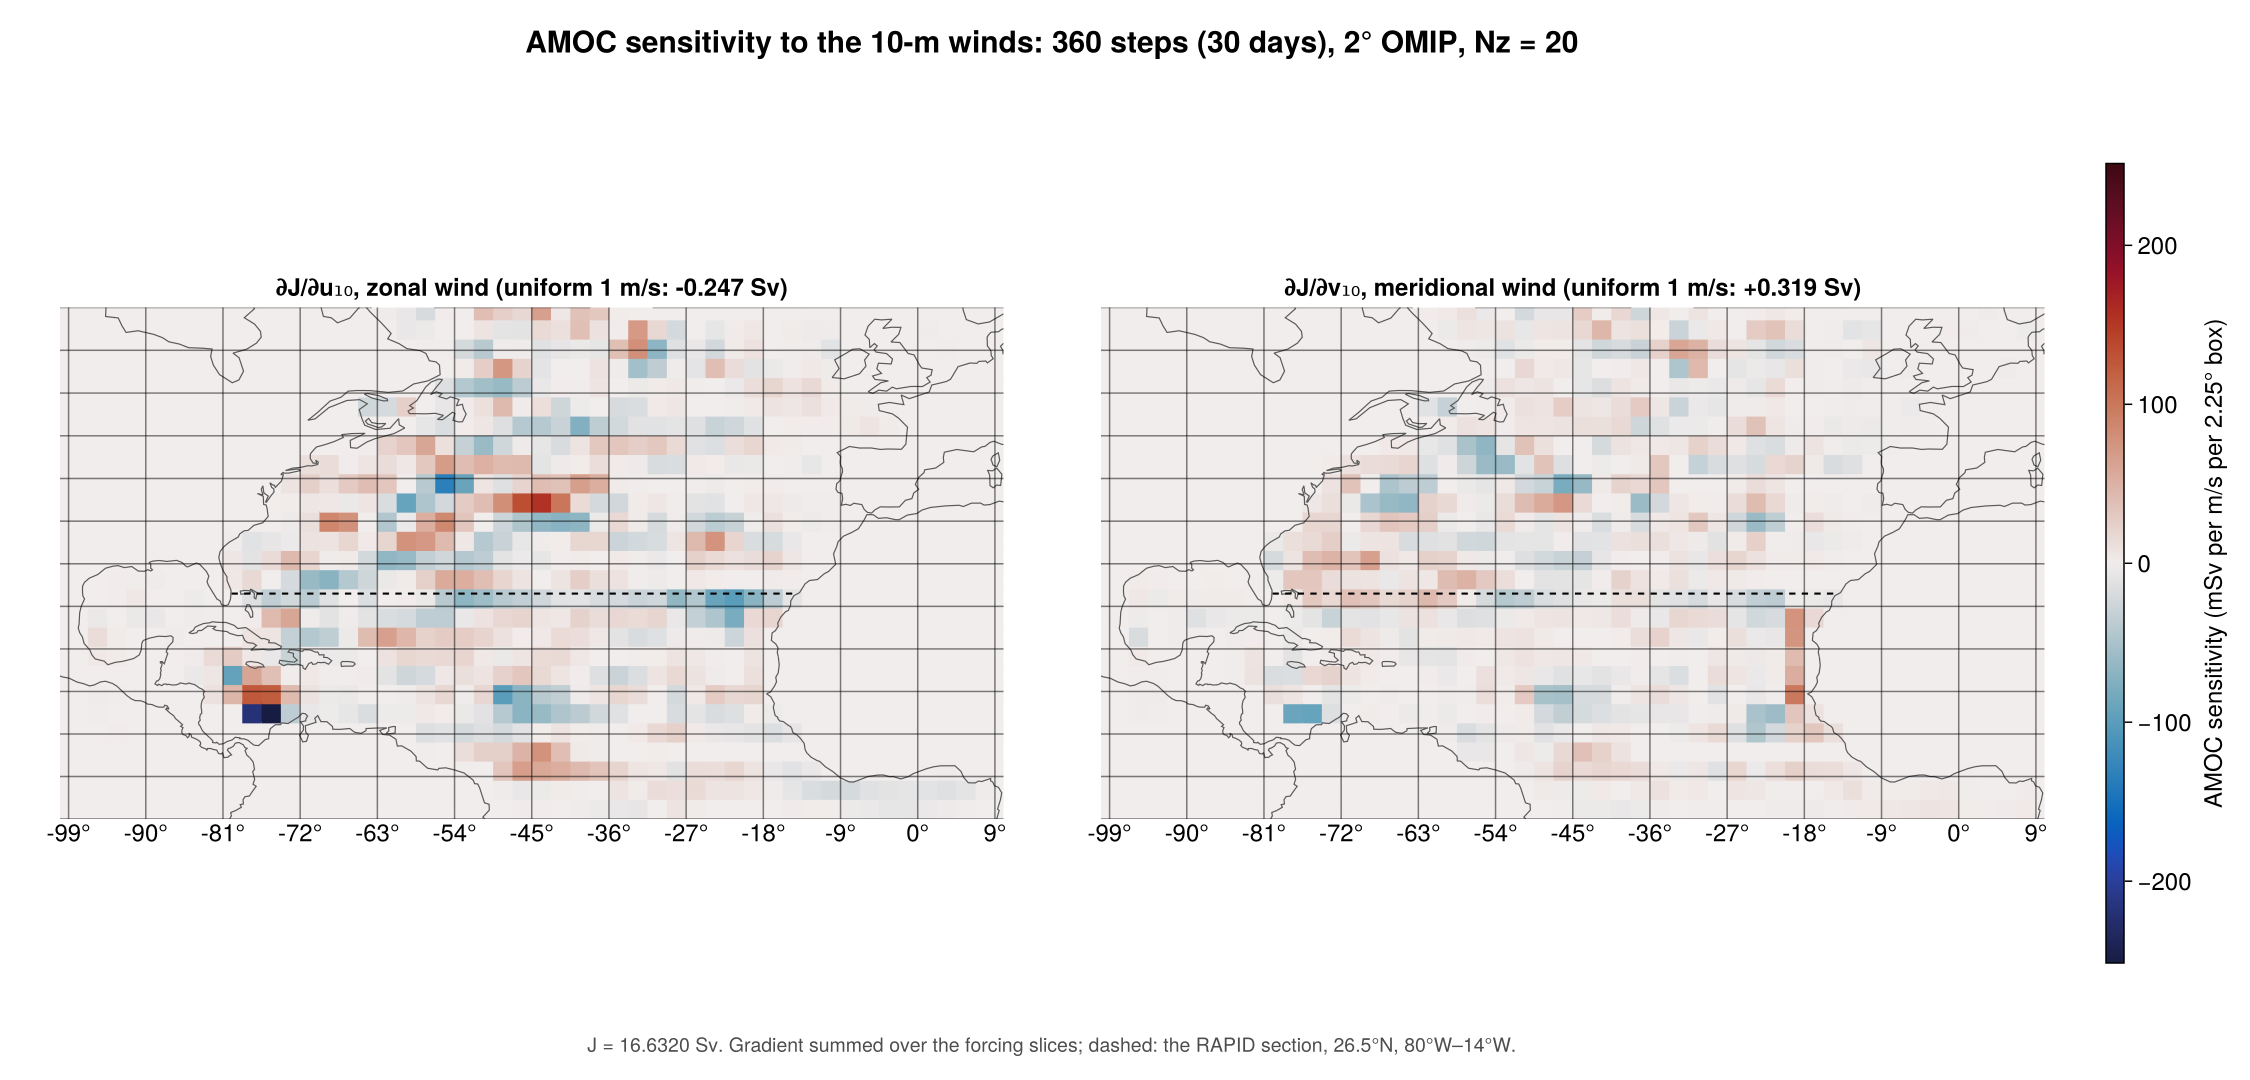
\includegraphics[width=0.8\textwidth,trim=0 60 0 40,clip]{figures/amoc_sensitivity_twodegree_nz20_360step.png}
\caption{Sensitivity of $J$ after 30 days to the zonal and meridional \SI{10}{m} wind, summed over the window's
forcing slices, in \ang{2.25} boxes. Dashed: the RAPID section.}
\label{fig:wind}
\end{figure}

After one week the zonal-wind sensitivity lies in zonal bands along and just south of the section (Ekman
transport), and the meridional-wind sensitivity at the African coast near \ang{18}W. By 30 days
(Fig.~\ref{fig:wind}) the pattern has broken into isolated boxes, the largest in the Caribbean. These windows start
from rest, so they sample the adjustment from rest, not an equilibrium sensitivity.

\subsection{Lead-time sensitivity over 90 days (forcing B, frozen mixing)}

\begin{figure}[H]
\centering
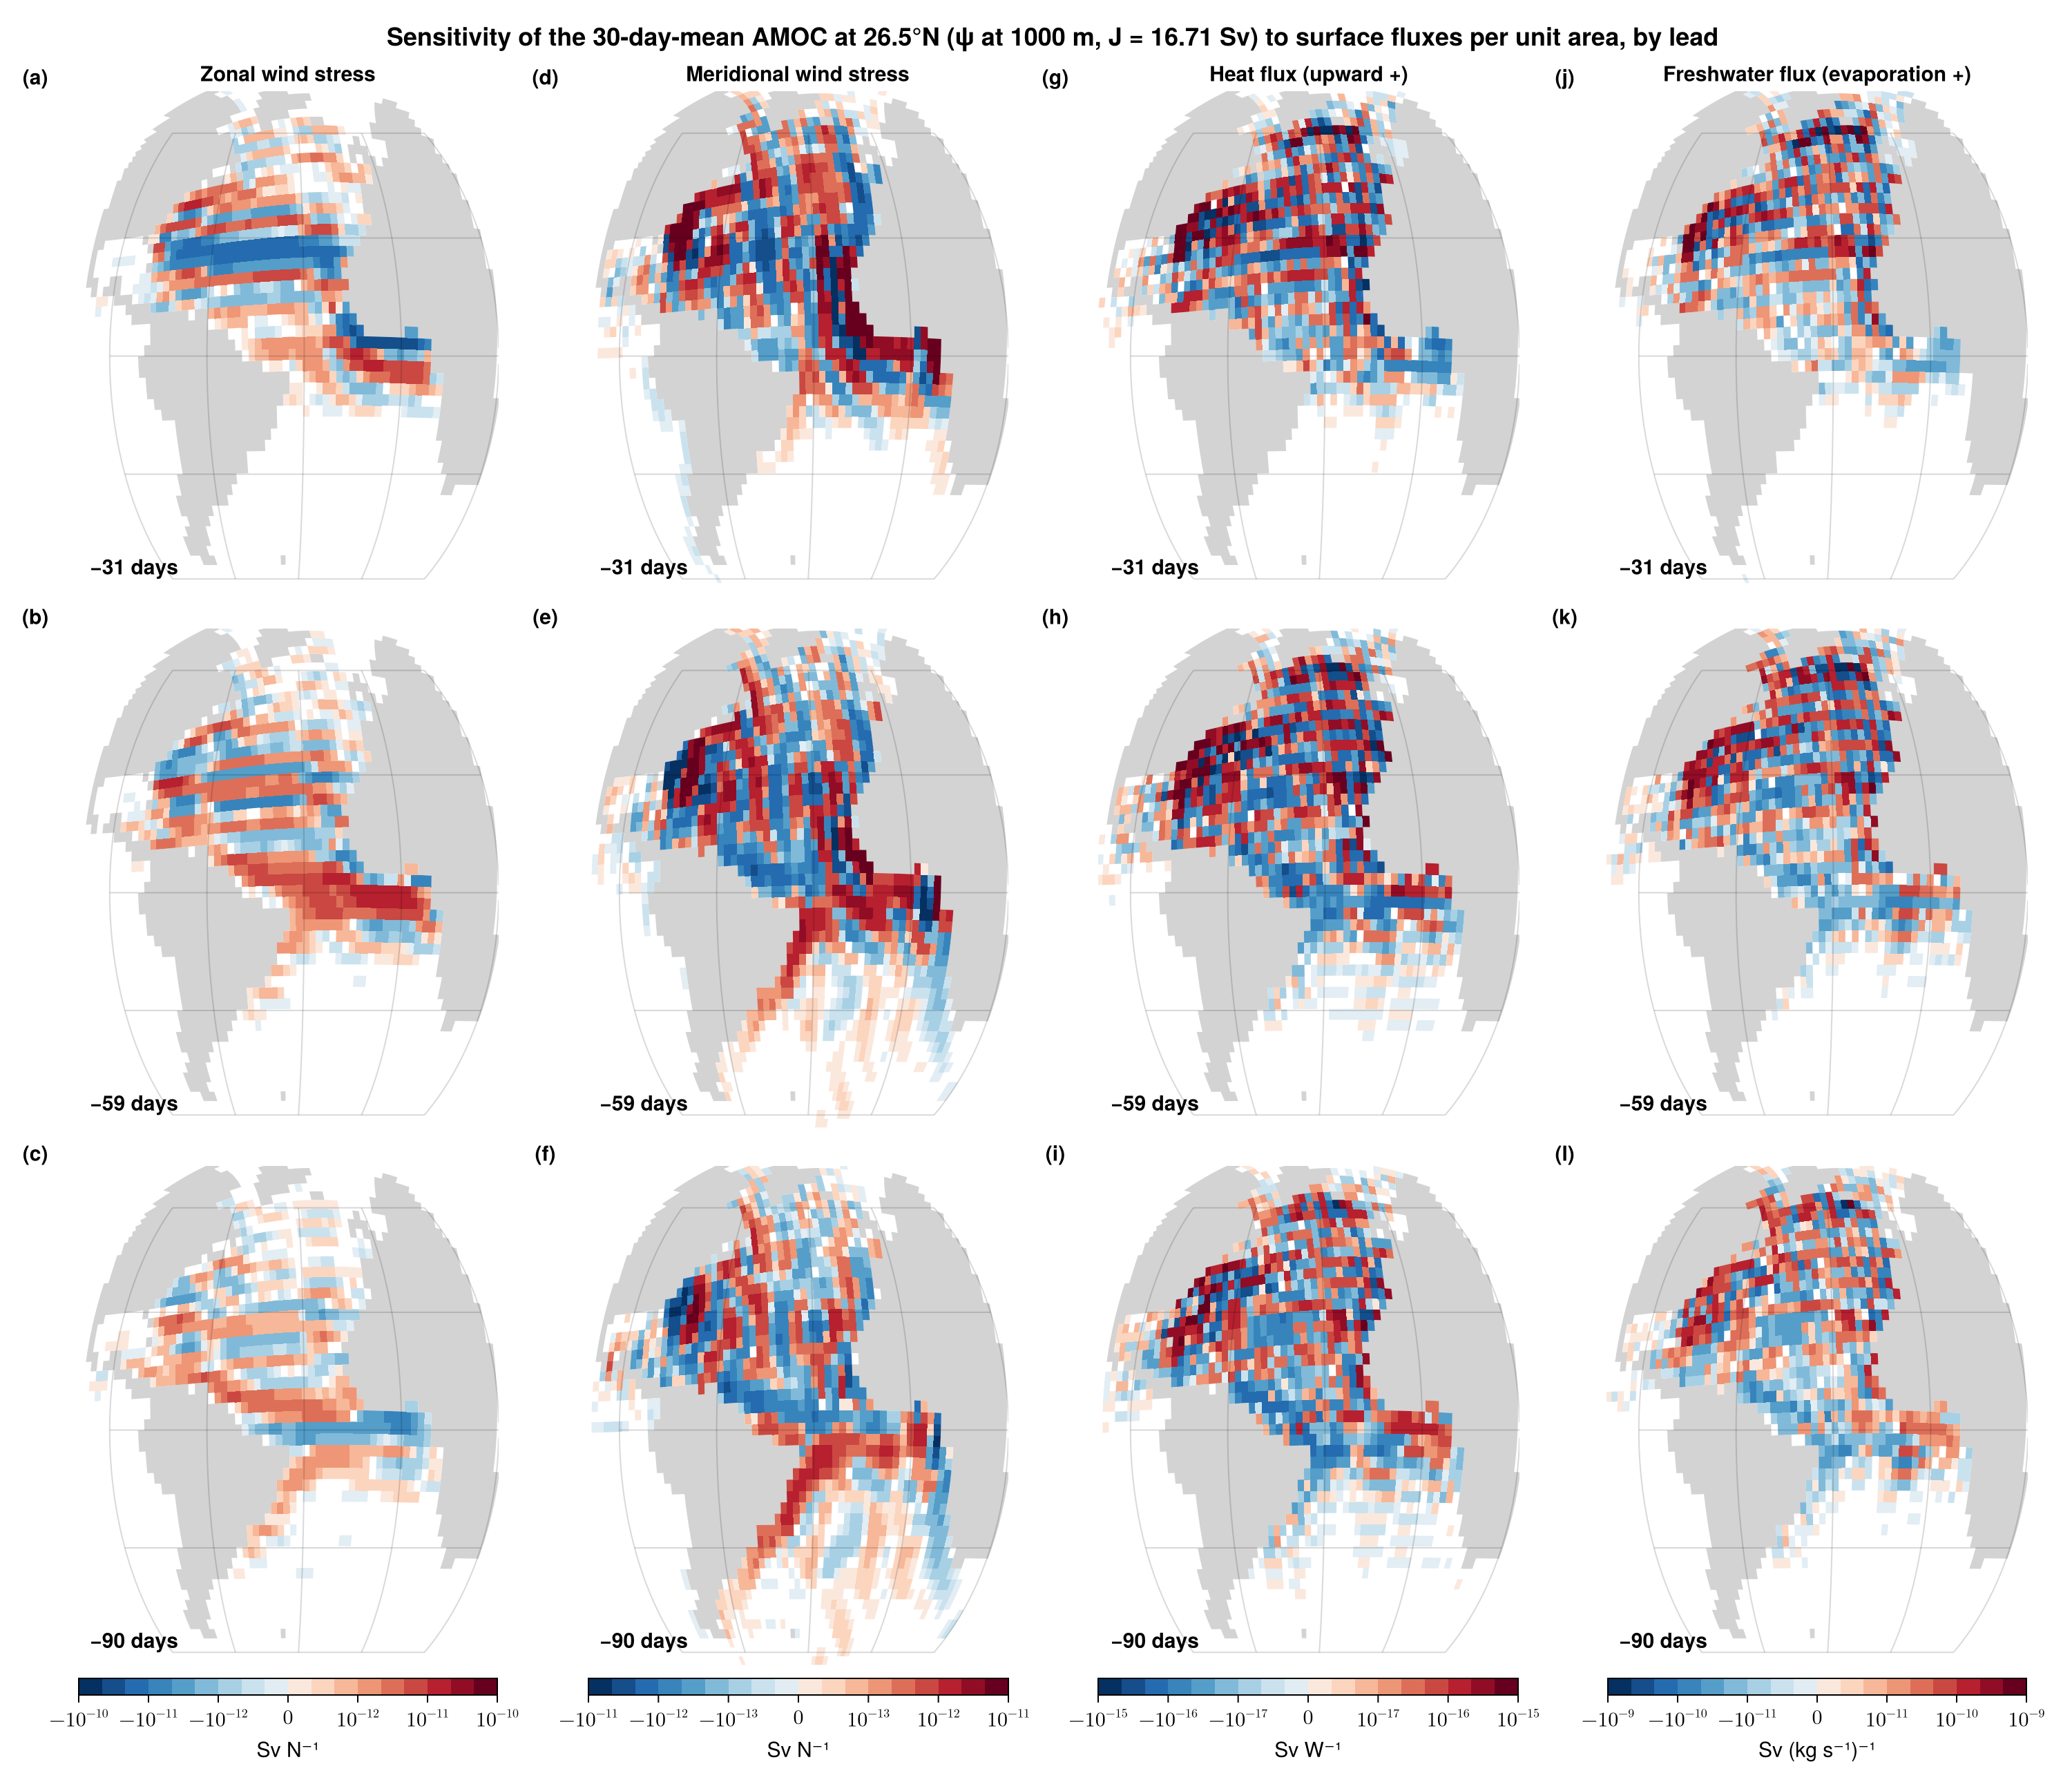
\includegraphics[width=0.74\textwidth]{figures/lead_sensitivity_ecco4_nz20_90day_frozen.png}
\caption{Sensitivity of the 30-day-mean AMOC (days 61--90, $J = \SI{16.71}{Sv}$) to each monthly flux slice, per unit
area, by lead (rows) and forcing (columns), after Pillar et al.\ (2016, Fig.~1). Signs follow Pillar: upward heat flux
and evaporation are positive. Colors are logarithmic over three decades.}
\label{fig:lead}
\end{figure}

At a one-month lead the zonal-stress sensitivity lies in zonal bands at and north of the section, the local Ekman
response. The meridional-stress sensitivity lies along the western boundary, the African coast and the equator, and
spreads into the tropics and South Atlantic with longer lead, as in Pillar's $-1$ and $-3$ month rows. Stress
magnitudes, about \SI{e-10}{Sv} per N, match ReactOcean's 90-day maps. The heat- and freshwater-flux columns show
the cell-scale checkerboard ReactOcean also found, and should not be interpreted yet.

\section{Longer windows: an instability of the linearized model}

\begin{figure}[H]
\centering
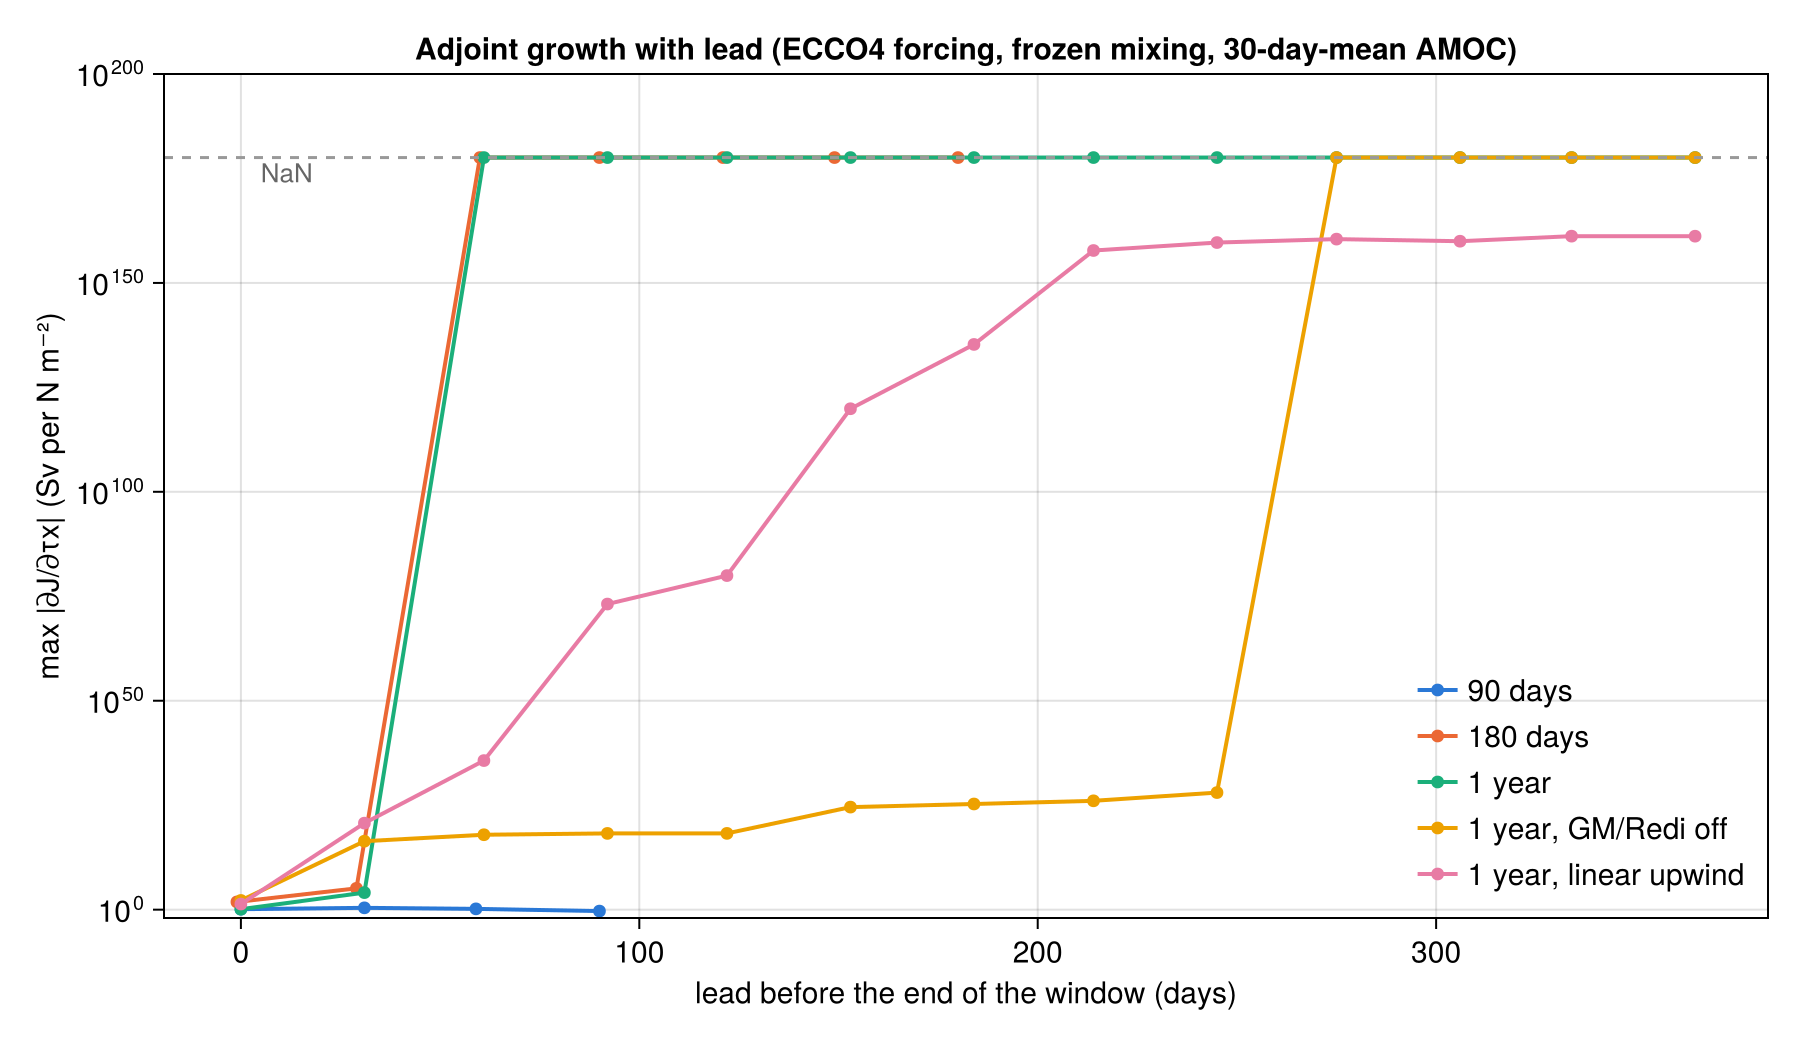
\includegraphics[width=0.72\textwidth]{figures/lead_growth_ecco4_nz20.png}
\caption{Largest $|\partial J/\partial\tau_x|$ over cells for each monthly slice, against lead, for forcing B with
frozen mixing. Points on the dashed line are NaN.}
\label{fig:growth}
\end{figure}

The 90-day window is healthy (values of order one at every lead). Every longer window grows by roughly one e-fold
every \SI{17}{h} backward in time, beginning within a month of its end, and reaches NaN by two months
(Fig.~\ref{fig:growth}). The tests so far each change one thing:
\begin{itemize}
  \item \textbf{Window ending in June} (180 days) instead of December (1 year): the same growth, so it is not tied
        to the autumn state.
  \item \textbf{GM/Redi off:} slower at first but still about $10^{16}$ per month, and NaN beyond eight months.
  \item \textbf{WENO replaced by linear third-order upwind:} no NaN, but steady growth to $10^{161}$.
\end{itemize}
So no single adjoint term is responsible. The forward model stays bounded throughout. Some nonlinearity therefore
keeps finite perturbations in check while infinitesimal ones grow, consistent with the jumps of
Fig.~\ref{fig:fd}.

\textbf{Forward health check.} To see what changes in the forward run, the 180-day window was stepped with the same
compiled step, recording diagnostics every 5 days (Fig.~\ref{fig:health}).
\begin{itemize}
  \item \textbf{CFL numbers stay small:} vertical $\le 0.03$ and horizontal $\le 0.07$ after spin-up. The time step
        does not appear to be the cause; a $\Delta t = \SI{1}{h}$ run is queued to confirm.
  \item \textbf{SST drifts} away from ECCO4 to \SI{3.1}{\celsius} rms by day 180. ECCO4's prescribed fluxes do not
        respond to SST, so nothing pulls the model back.
  \item \textbf{Grid-scale surface temperature noise} (the field minus its four-neighbor mean) grows steadily, from
        \SI{0.26}{K} to \SI{0.66}{K} rms, with single cells 11--\SI{14}{K} off their neighbors. It concentrates where
        the adjoint explodes: the Gulf Stream and North Atlantic Current, the subpolar North Atlantic, the Kuroshio and
        the western equatorial Pacific. It also forms zonal stripes along tripolar rows in the Pacific.
  \item \textbf{Statically unstable interfaces} rise to about 4900 after day 90, and CATKE's diffusivity sits at its
        \SI{3}{m^2/s} cap in winter convective regions.
\end{itemize}

\begin{figure}[H]
\centering
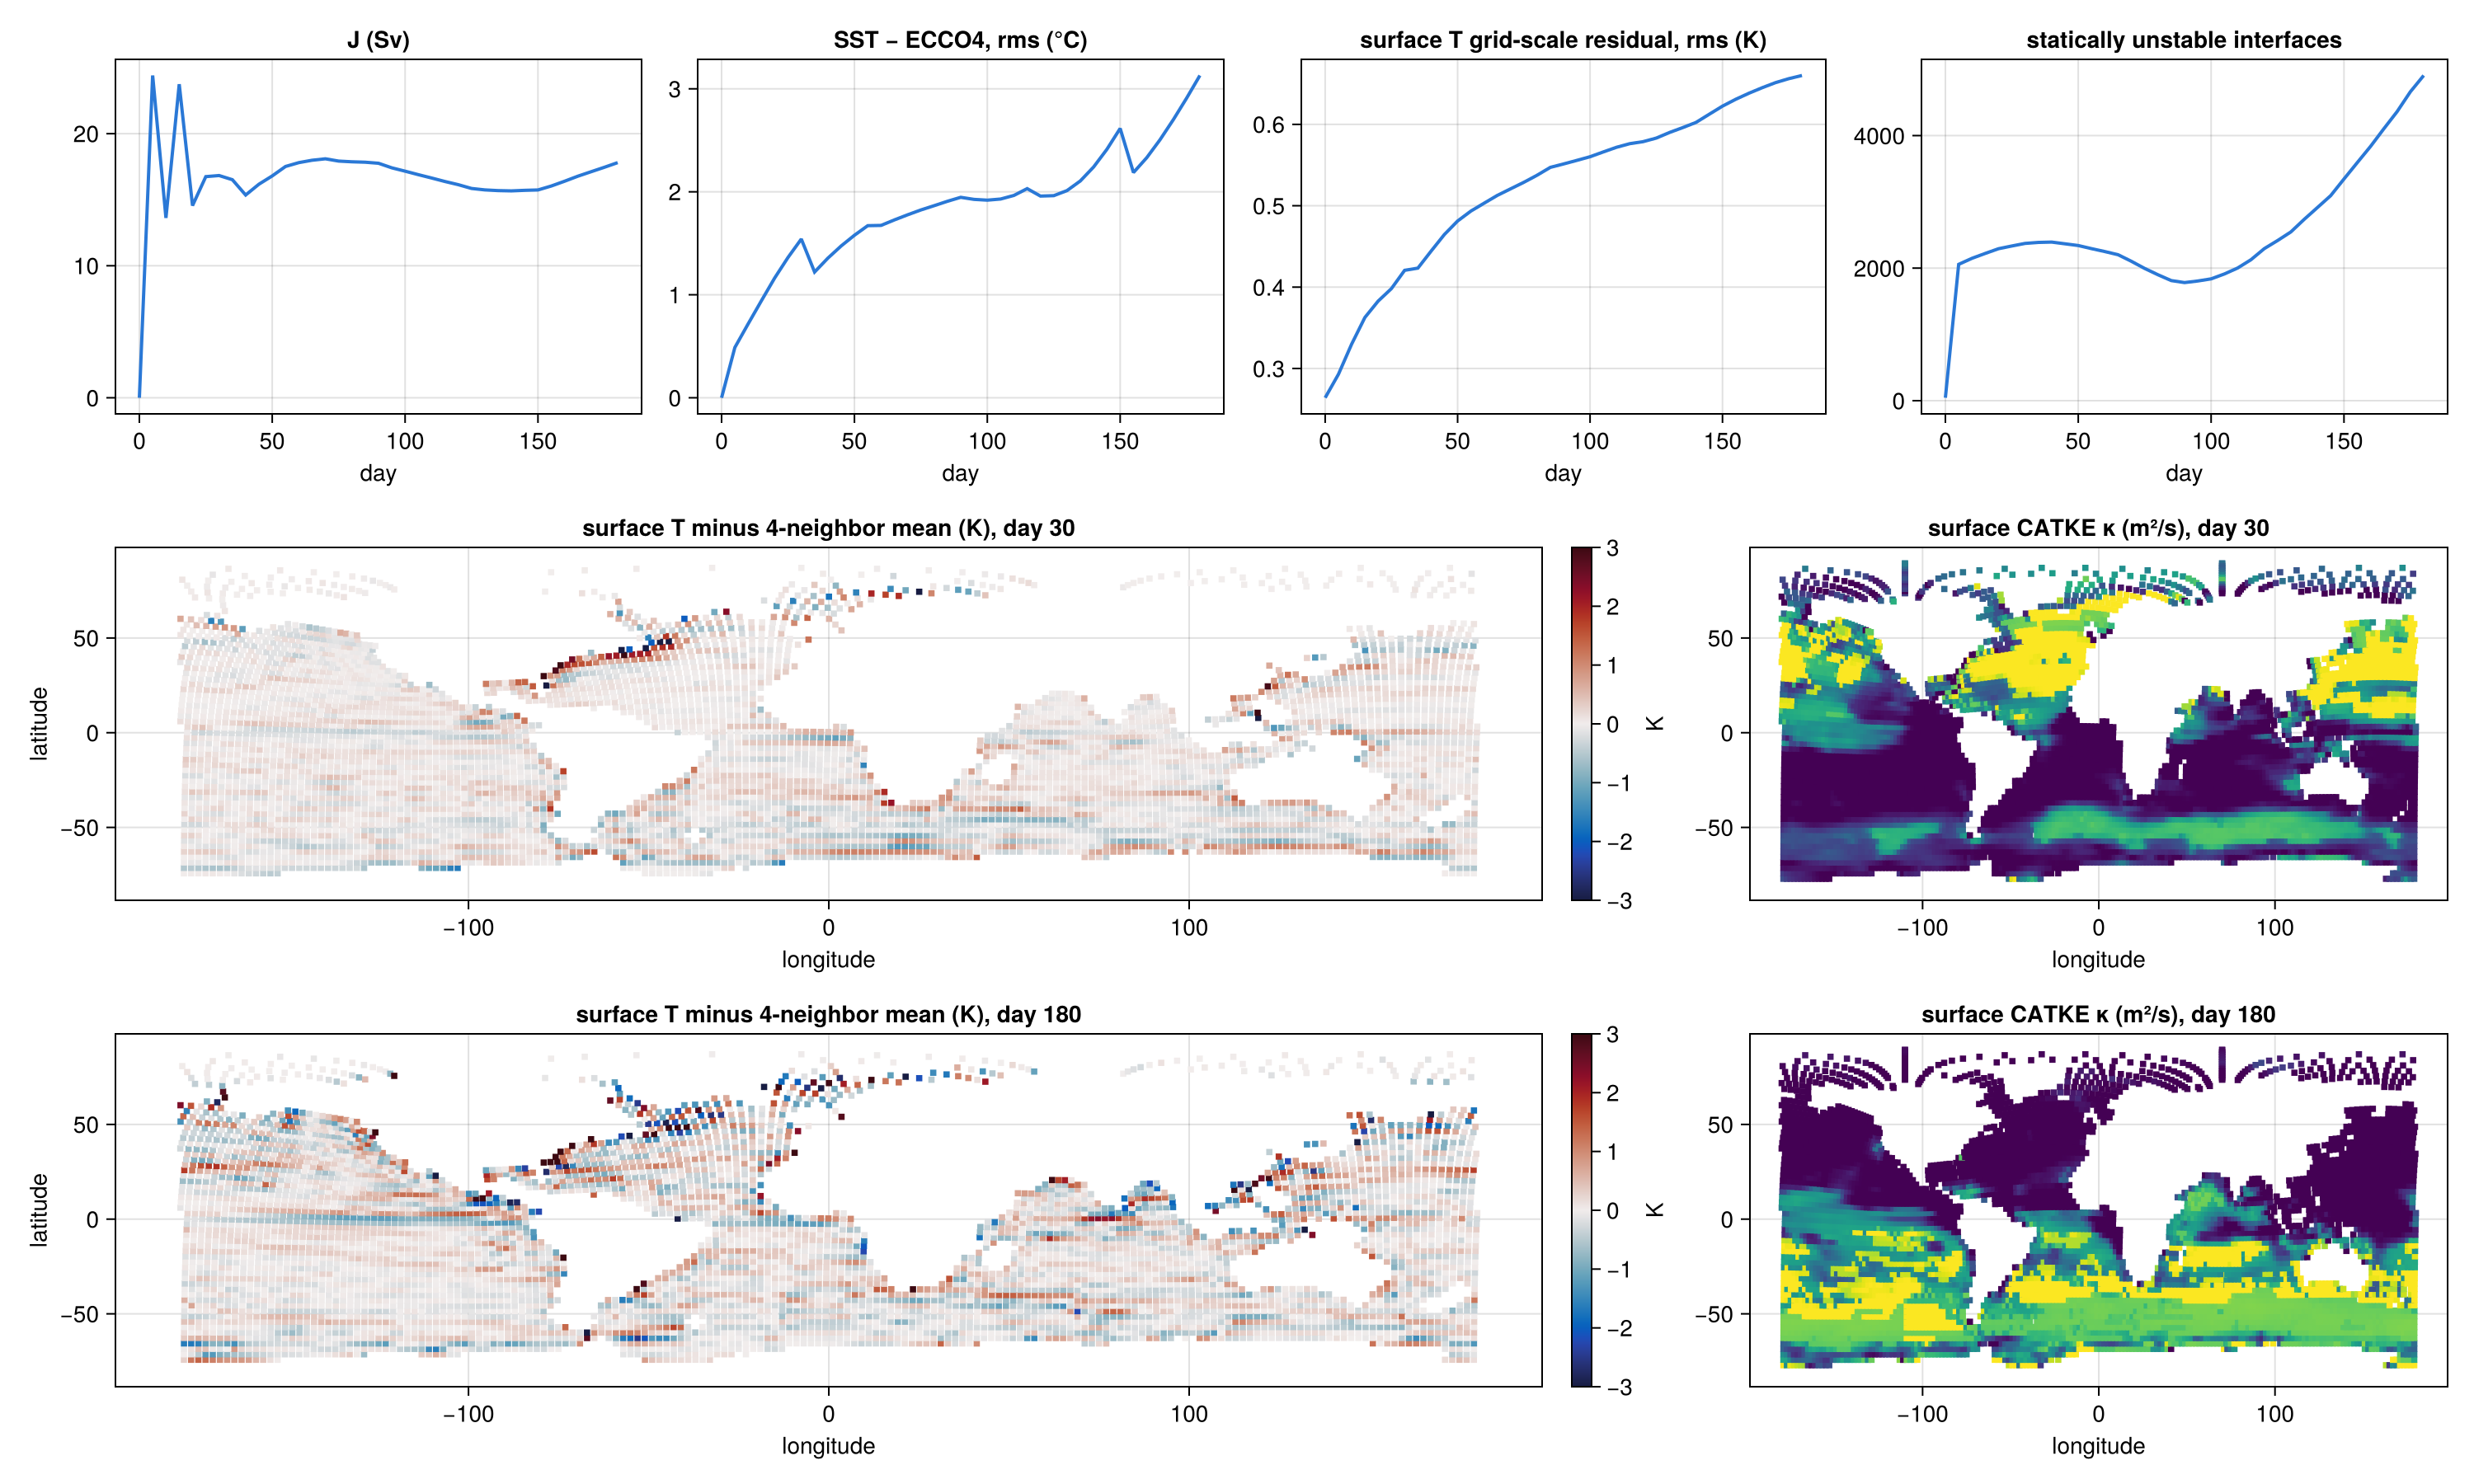
\includegraphics[width=0.95\textwidth]{figures/forward_health_ecco4_nz20_180day.png}
\caption{Forward health of the 180-day window (forcing B). Top: $J$, rms SST error against ECCO4, rms grid-scale
surface temperature residual, and the number of statically unstable interfaces. Middle and bottom: the surface
grid-scale temperature residual and CATKE's surface diffusivity at days 30 and 180.}
\label{fig:health}
\end{figure}

A noisy, drifting forward state is the kind a linearized model can amplify enormously while the forward model
limits itself. This points to the forward configuration (fixed fluxes, no explicit horizontal tracer diffusion)
rather than the adjoint machinery.

\section{Software and infrastructure}

\textbf{Oceananigans 0.117.2.} NumericalEarth's OMIP branch moved from a deleted Oceananigans development branch
(0.113.5) to the registered 0.117.2. That release includes the fix for a Reactant adjoint bug on the tripolar fold
(CliMA/Oceananigans.jl\#6396). The merged OMIP code also patches two other fold bugs: the buoyancy-gradient sign, and
the T-pivot vertical halos. Of the 13 OMIP feature branches, 8 are in 0.117.2. The one that matters for us, high-order WENO
boundary reconstruction (\#5932), is not, so advection near boundaries now falls back to a low-order upwind buffer.
$J$ moves by \SI{0.17}{\percent}, and the adjoint still verifies (Section~\ref{sec:verification}). ReactOcean, the
companion code, is on the same versions: Oceananigans 0.117.2, Reactant 0.2.303, Enzyme 0.13.216.

\textbf{Julia 1.13.} Under Julia 1.13.3 nothing compiles with Reactant 0.2.303. The newer LLVM emits unsigned
integer-to-float conversions that Reactant's XLA export rejects (\texttt{arith.uitofp}). The CPU model is
unaffected, so the GPU runs stay on Julia 1.12.7.

\textbf{Reactant and Enzyme issues.} Eight are recorded with evidence and workarounds. Only the tripolar-fold one has
been reported upstream (EnzymeAD/Reactant.jl\#3636). The others:
\begin{itemize}
  \item zero-valued loop-carried shadow state in Enzyme-JAX (\SI{73}{GiB});
  \item two rewrite patterns (\texttt{while\_deadresult}, \texttt{cse\_reduce\_transposed}) that cost tens of
        minutes of compile time;
  \item \texttt{WHILE\_UNROLL\_THRESHOLD} acting after differentiation;
  \item the aarch64 ``fixup value out of range'' failure that keeps gradients off Vista;
  \item the 13--\SI{40}{min} first-call cost;
  \item the Julia 1.13 export failure.
\end{itemize}

\section{Next steps and decisions}
\label{sec:next}

\begin{enumerate}
  \item \textbf{Decision: stabilize the forward state for long windows.} The options are
        \begin{enumerate}[label=(\alph*)]
          \item SST/SSS feedback on the ECCO4 fluxes, $\lambda(\mathrm{SST}_{\mathrm{ECCO}} - \mathrm{SST})$ with
                $\lambda \approx \SI{40}{W\,m^{-2}\,K^{-1}}$ (standard with prescribed fluxes; removes the drift, but
                makes the heat-flux control less pure);
          \item explicit horizontal tracer diffusion of \SIrange{500}{1000}{m^2/s} on top of WENO, as in ECCOv4, to
                damp the grid-scale noise in both models;
          \item both.
        \end{enumerate}
        Each is one configuration switch and one 1-year run.
  \item \textbf{Queued:} \ang{1} windows of 90 days and 1 year on H100 (does resolution change the growth?), and
        $\Delta t = \SI{1}{h}$ at \ang{2} (does the time step?).
  \item Finite differences along uniform-wind directions, to settle the full- versus frozen-mixing large-scale
        sums.
  \item Then a spun-up initial state instead of rest, Nz = 70, and one-year lead-time maps after Pillar et al.
\end{enumerate}

\end{document}
